\documentclass[12pt,letterpaper,oneside]{book}

\usepackage[utf8]{inputenc}

% Paquete con configuraciones necesarias para cambiar el margen de las páginas
\usepackage[left=1.5cm, right=1.5cm, top=2.5cm, bottom=2.5cm]{geometry}
% - - - - - - - - - - - - - - - - - - - - - - - - - - - - - - - - - - - - - -

% Paquete necesario para incluir una imagen en el documento
\usepackage{graphicx}
% - - - - - - - - - - - - - - - - - - - - - - - - - - - - - - - - - - - - - -

%Paquete necesario para utilizar algunas funcionalidades avanzadas en ecuaciones
\usepackage{amsmath}
% - - - - - - - - - - - - - - - - - - - - - - - - - - - - - - - - - - - - - -

\title{Documentación de una fórmula}
\author{Emilio-Ernesto Hernández-Huerfano}

\begin{document}

\maketitle
% Primer capítulo
\chapter{Formula del Semiverseno}
\noindent La \textbf{fórmula de Haversine}\footnote{\textit{Haversine} viene como una contracción de Half-Versine.} o del Semiverseno es una importante ecuación para la navegación astronómica, en cuanto al cálculo de la distancia de círculo máximo entre dos puntos de un globo (figura \ref{fig:haversine}) sabiendo su longitud ($\lambda$) y su latitud ($\phi$).


\begin{figure}[h]
\centering
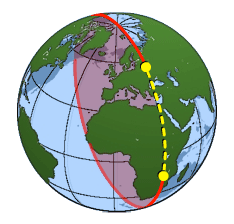
\includegraphics[scale=.8]{img/haversine.png}
\caption{Cálculo de la distancia entre dos puntos $(\phi, \lambda)$}
\label{fig:haversine}
\end{figure}

%En esta parte podrías meter algo acerca de la contraindicación en el uso de la distancia euclidiana sobre superficies curvas

\section{Formulación}
La distancia $d$ que existe entre dos puntos $(\phi, \lambda)$ está dada por la siguiente fórmula:$$d=R \cdot c$$

en donde:
\begin{itemize}
\item $R \Rightarrow$  radio ecuatorial asignado al planeta tierra: 6378.1km
\item $c \Rightarrow$ es un coeficiente de distancia que está dado por la formula \ref{eq:haversine}.
\end{itemize}

\begin{equation} \label{eq:haversine}
\begin{split}
c & = 2 \cdot \arctan (\sqrt{a} ,\sqrt{1-a} )^{2} \\
a & = \sin(\frac{\Delta\phi}{2})^{2} + \cos(\phi 1) \cdot \cos(\phi 2) \cdot \sin(\frac{\Delta\lambda}{2})^{2} 
\end{split}
\end{equation}

Donde:
\begin{itemize}
\item $\Delta\lambda \Rightarrow$ es la diferencia entre longitudes ($\lambda$).
\item $\Delta\phi \Rightarrow$ es la diferencia entre latitudes ($\phi$).
\end{itemize}

\end{document} 